
\chapter{The Eletronics} \label{chap:conc}

In order for the aircraft to fly and navigate autonomously, onboard electronics are required, for both actuation, power source, and navigation. Some of the used electronics was already available, and was chosen for this reason.
	
\section{Propulsion}

Due to the familiriaty and availability, the Mikrokopter Mk3538 Motor was chosen, paired with E-Max Simon 60A escs.

Experimental curves for the motor are available at Mikrokopter's website, and the relevant ones are reproduced on Figure \ref{fig:motorcurves}. Each motor should give, on 25 V, at least 2.2kg of static thrust when paired to 12 inches propellers, up to 3.4 kg on 15 inches, while drawing 34 A, or about 754 W.
\begin{figure}
\centering
  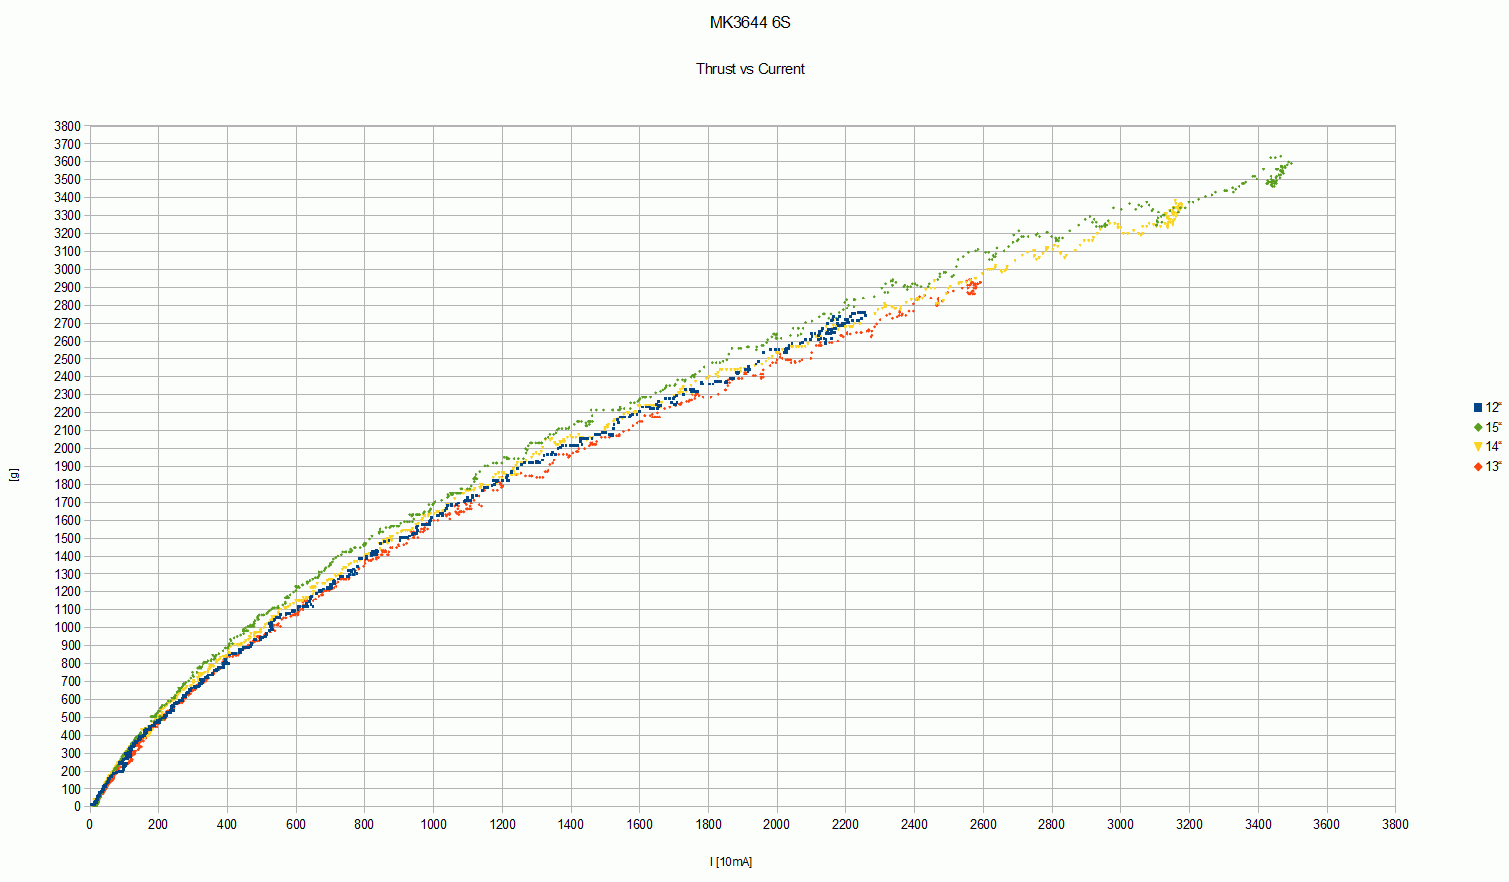
\includegraphics[width=\linewidth]{figs/motorcurves.png}
  \caption{First concept of the aircraft.}
  \label{fig:motorcurves}
\end{figure}


\section{Batteries}

As each motor can draw up to 34 A, the battery should be able to provide up to 68 A without issues.
The Batteries chosen are also the ones already in use by the company, XXX which, at XX C rating, are able to sustain a constant draw of up to XX A. \todo{tamanho da bateria?}.

Each weigh aproximately XXXX g and 

\section{The Control Surfaces}

The control surfaces must be slightly larger than usual for a flying wing, as on a tail-sitter a reasonable ammount of air must be deflected on hover situation, while on most wings a steady airflow is assumed.

\section{The Flight Controller}

The Flight Controller is a PixHawk, running latest Beta release of ArduPlane, where there's experimental support for tail-sitters.


%%%%%%%%%%%%%%%%%%%